\documentclass{beamer}

\usepackage{comment}
\usepackage{color}
\usepackage{listings}
\usepackage{verbatim}
\usepackage{multicol}
\usepackage{booktabs}
\definecolor{green}{RGB}{0,128,0}

\def\EQ#1\EN{\begin{equation*}#1\end{equation*}}
\def\BA#1\EA{\begin{align*}#1\end{align*}}
\def\BS#1\ES{\begin{split*}#1\end{split*}}
\newcommand{\bc}{\begin{center}}
\newcommand{\ec}{\end{center}}
\newcommand{\eq}{\ =\ }
\newcommand{\degc}{$^\circ$C}

\def\p{\partial}
\def\qbs{\boldsymbol{q}}
\def\Dbs{\boldsymbol{D}}
\def\A{\mathcal A}
\def\gC{\mathcal C}
\def\gD{\mathcal D}
\def\gL{\mathcal L}
\def\M{\mathcal M}
\def\P{\mathcal P}
\def\Q{\mathcal Q}
\def\gR{\mathcal R}
\def\gS{\mathcal S}
\def\X{\mathcal X}
\def\bnabla{\boldsymbol{\nabla}}
\def\bnu{\boldsymbol{\nu}}
\renewcommand{\a}{{\alpha}}
%\renewcommand{\a}{{}}
\newcommand{\s}{{\sigma}}
\newcommand{\bq}{\boldsymbol{q}}
\newcommand{\bz}{\boldsymbol{z}}
\def\bPsi{\boldsymbol{\Psi}}

\def\Li{\textit{L}}
\def\Fb{\textbf{f}}
\def\Jb{\textbf{J}}
\def\cb{\textbf{c}}

\def\Dt{\Delta t}
\def\tpdt{{t + \Delta t}}
\def\bpsi{\boldsymbol{\psi}}
\def\dbpsi{\delta \boldsymbol{\psi}}
\def\bc{\textbf{c}}
\def\dbc{\delta \textbf{c}}
\def\arrows{\rightleftharpoons}

\newcommand{\bGamma}{\boldsymbol{\Gamma}}
\newcommand{\bOmega}{\boldsymbol{\Omega}}
%\newcommand{\bPsi}{\boldsymbol{\Psi}}
%\newcommand{\bpsi}{\boldsymbol{\psi}}
\newcommand{\bO}{\boldsymbol{O}}
%\newcommand{\bnu}{\boldsymbol{\nu}}
\newcommand{\bdS}{\boldsymbol{dS}}
\newcommand{\bg}{\boldsymbol{g}}
\newcommand{\bk}{\boldsymbol{k}}
%\newcommand{\bq}{\boldsymbol{q}}
\newcommand{\br}{\boldsymbol{r}}
\newcommand{\bR}{\boldsymbol{R}}
\newcommand{\bS}{\boldsymbol{S}}
\newcommand{\bu}{\boldsymbol{u}}
\newcommand{\bv}{\boldsymbol{v}}
%\newcommand{\bz}{\boldsymbol{z}}
\newcommand{\pressure}{P}

\def\water{H$_2$O}
\def\calcium{Ca$^{2+}$}
\def\copper{Cu$^{2+}$}
\def\magnesium{Mg$^{2+}$}
\def\sodium{Na$^+$}
\def\potassium{K$^+$}
\def\uranium{UO$_2^{2+}$}
\def\hion{H$^+$}
\def\hydroxide{0H$^-$}
\def\bicarbonate{HCO$_3^-$}
\def\carbonate{CO$_3^{2-}$}
\def\cotwo{CO$_2$(aq)}
\def\chloride{Cl$^-$}
\def\fluoride{F$^-$}
\def\phosphoricacid{HPO$_4^{2-}$}
\def\nitrate{NO$_3^-$}
\def\sulfate{SO$_4^{2-}$}
\def\souotwooh{$>$SOUO$_2$OH}
\def\sohuotwocothree{$>$SOHUO$_2$CO$_3$}
\def\soh{$>$SOH}

\newcommand\gehcomment[1]{{{\color{orange} #1}}}
\newcommand\add[1]{{{\color{blue} #1}}}
\newcommand\remove[1]{\sout{{\color{red} #1}}}
\newcommand\codecomment[1]{{{\color{green} #1}}}
\newcommand\redcomment[1]{{{\color{red} #1}}}
\newcommand\bluecomment[1]{{{\color{blue} #1}}}
\newcommand\greencomment[1]{{{\color{green} #1}}}
\newcommand\magentacomment[1]{{{\color{magenta} #1}}}

\begin{comment}
\tiny
\scriptsize
\footnotesize
\small
\normalsize
\large
\Large
\LARGE
\huge
\Huge
\end{comment}

\begin{document}
\title{Gridded Datasets as Boundary Conditions}
\author{Jenn Frederick}
\date{\today}

%\frame{\titlepage}

%-----------------------------------------------------------------------------
\section{Location of Example}

\begin{frame}[fragile,containsverbatim]\frametitle{Location}

Location of this example problem:

\begin{semiverbatim}
> cd \$PFLOTRAN_DIR
> cd shortcourse/exercises/gridded_datasets
> ls

2D_steady_pressure_BC_1st_2nd_kind.in
create_dataset.py
\end{semiverbatim}

\end{frame}

%-----------------------------------------------------------------------------
\section{The Test Problem Description}

\begin{frame}[fragile,containsverbatim]\frametitle{Problem Description}

This is one of PFLOTRAN's QA tests (2D Steady Flow, BCs of 1st (Dirichlet) and 2nd (Neumann) kind).
  \begin{itemize}
    \item Domain: 2x1x1 m rectangular slab
    \item Grid cells: 20x10x1 hexahedral cells; dimensions 0.1x0.1x1 m
    \item Single material:
    \begin{itemize}
      \item k = 1 $\times$ 10$^{-14}$ m$^{2}$
      \item $\phi$ = 0.50
    \end{itemize}
    \item Constant fluid properties:
    \begin{itemize}
      \item $\rho_{f}$ = 1000 kg/m$^{3}$
      \item $\mu_{f}$ = 1 mPa-s
    \end{itemize}
    \item Initial Conditions:
    \begin{itemize}
      \item P(x,y,t=0) = 1.0 MPa
    \end{itemize}
    
  \end{itemize}

\end{frame}

%-----------------------------------------------------------------------------
\begin{frame}[fragile,containsverbatim]\frametitle{Problem Description}

This is one of PFLOTRAN's QA tests (2D Steady Flow, BCs of 1st 2nd kind).

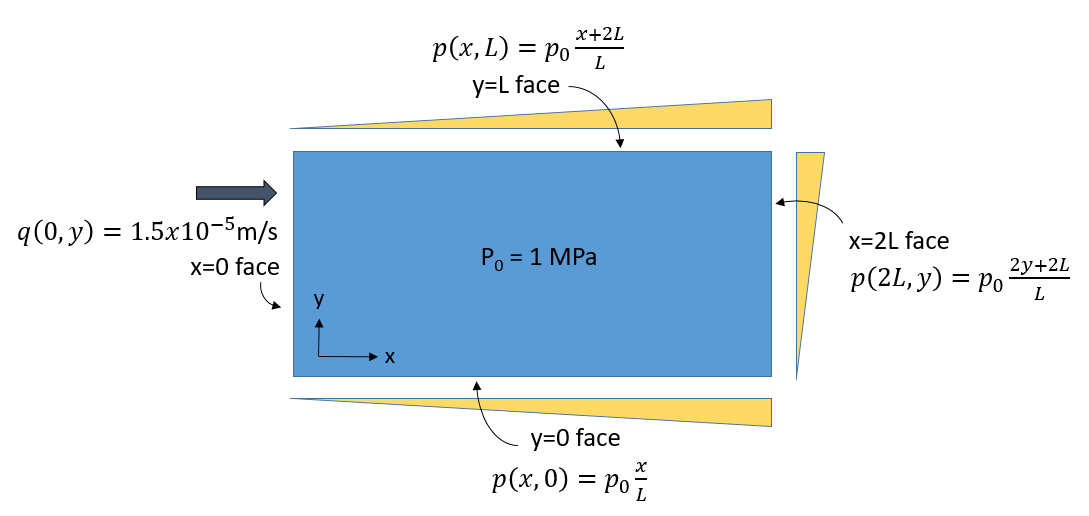
\includegraphics[width=1.2\textheight]{./BC_schematic.png}

L = 1 m

\end{frame}

%-----------------------------------------------------------------------------
\begin{frame}[fragile,containsverbatim]\frametitle{Problem Description}

The steady-state solution is governed by the LaPlace equation:
\Large 
\vspace{0.25 in}
${{\partial^{2} p} \over {\partial x^{2}}} + {{\partial^{2} p} \over {\partial y^{2}}} = 0$ 
  
\vspace{0.50 in}  
\normalsize  
When the boundary conditions are applied, the solution is:
\Large 
\vspace{0.25 in}
$p(x,y) = {p_0 \over L} (x+2y)$

\end{frame}

%-----------------------------------------------------------------------------
\begin{frame}[fragile,containsverbatim]\frametitle{Problem Description}

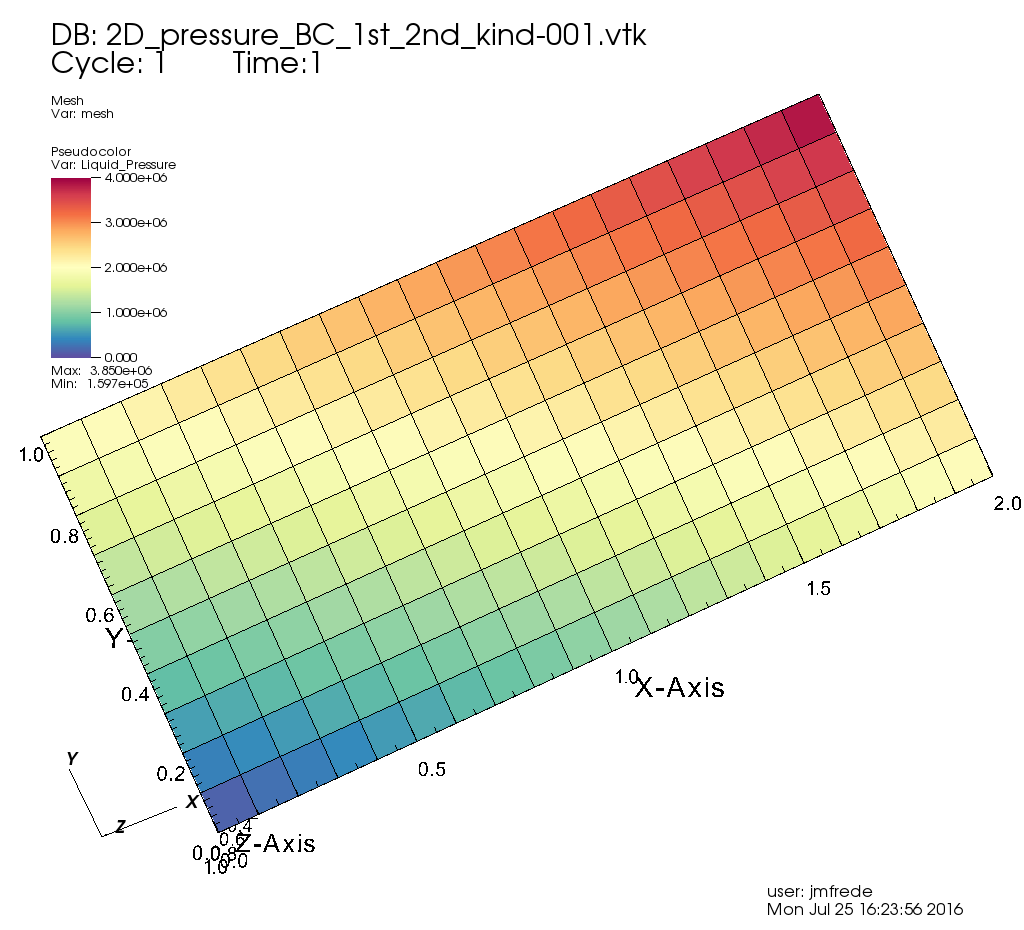
\includegraphics[width=0.75\textheight]{./visit_figure.png}

\end{frame}

%-----------------------------------------------------------------------------
\begin{frame}[fragile,containsverbatim]\frametitle{Problem Description}

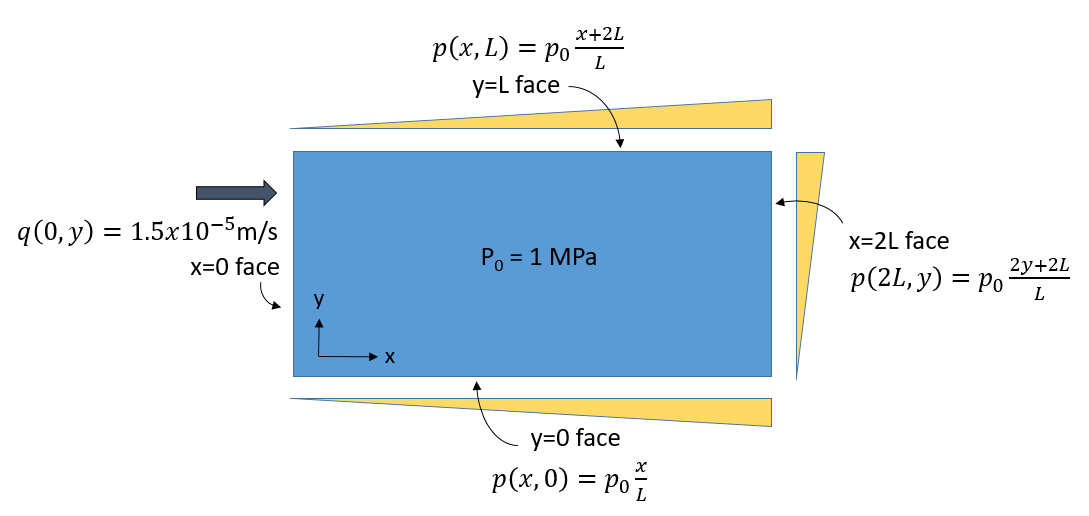
\includegraphics[width=1.2\textheight]{./BC_schematic.png}

How do we apply these more complex boundary conditions? 

With a gridded dataset!

\end{frame}

%-----------------------------------------------------------------------------
\subsection{GRIDDED DATASET}

\begin{frame}[fragile,containsverbatim]\frametitle{Creating and Using a Gridded Dataset}

To apply the boundary conditions, we use a gridded dataset.

The datasets are HDF5 files, and they can be created with a python script.
To create the dataset, run the python script:

\begin{semiverbatim}
> cd \$PFLOTRAN_DIR
> cd shortcourse/exercises/gridded_datasets
> python create_dataset.py
\end{semiverbatim}

\end{frame}

%-----------------------------------------------------------------------------
\begin{frame}[fragile,containsverbatim]\frametitle{Creating and Using a Gridded Dataset}

The script will create a file called:

\begin{semiverbatim}
dataset.h5
\end{semiverbatim}

It has 3 groups in it called:
\begin{itemize}
  \item x\_line\_node\_centered\_north
  \item x\_line\_node\_centered\_south
  \item y\_line\_node\_centered\_east
\end{itemize}

These are the north (y=L), south (y=0), and east (x=2L) boundary conditions.
The west boundary condition is a fluid flux (neumann BC) and does not need a
gridded dataset.
\end{frame}

%-----------------------------------------------------------------------------
\begin{frame}[fragile,containsverbatim]\frametitle{Creating and Using a Gridded Dataset}

Open up the dataset.h5 file:

\begin{semiverbatim}
> hdfview dataset.h5
\end{semiverbatim}

The values are calculated at the cell face nodes (not at cell face centers).
Therefore, there are $nx + 1$ and $ny + 1$ values.
PFLOTRAN interpolates to find the values at the face centers.

\end{frame}

%-----------------------------------------------------------------------------
\begin{frame}[fragile,containsverbatim]\frametitle{Creating and Using a Gridded Dataset}

Open up the create\_dataset.py file:

\end{frame}

%-----------------------------------------------------------------------------
\begin{frame}[fragile,containsverbatim]\frametitle{DATASET}

After you've created the gridded dataset,
how do you use the gridded dataset in the simulation? 

\begin{semiverbatim}
DATASET pressure_bc_north
  HDF5_DATASET_NAME x_line_node_centered_north
  FILENAME ./dataset.h5
END
\end{semiverbatim}

There should be a DATASET block for each dataset group.

\end{frame}

%-----------------------------------------------------------------------------
\begin{frame}[fragile,containsverbatim]\frametitle{FLOW\_CONDITION}

After declaring the dataset using the DATASET block, you can use it in
the FLOW\_CONDITION block.

\begin{semiverbatim}
FLOW_CONDITION north_face
  TYPE
    PRESSURE dirichlet
  /
  PRESSURE DATASET pressure_bc_north
END

BOUNDARY_CONDITION north_face
  REGION north_face
  FLOW_CONDITION north_face
END
\end{semiverbatim}

\end{frame}

%-----------------------------------------------------------------------------
\begin{frame}[fragile]\frametitle{Command Line}

\begin{semiverbatim}

 > cd \$PFLOTRAN_DIR
 > cd shortcourse/exercises/gridded_datasets/
 > pflotran -input_prefix 2D_steady_pressure_BC_1st_2nd_kind

\end{semiverbatim}

The output is in HDF5 format. You can use Paraview to visualize it.

\begin{semiverbatim}
> paraview
\end{semiverbatim}

\end{frame}




\end{document}
